% !TEX root = ../TensorOT.tex

\section{Introduction}
\label{sec-intro}

% \justin{Eventually this introduction will need to be expanded.  In particular, we'll need to put this work into a graphics context, remind less experienced readers what OT is in non-mathematical terms, etc.  And typically SIGGRAPH papers have a figure on the first page.  I'm happy to write this once we have a better idea what our target applications will be.} \gabriel{I fully agree, your help will be much helpful/appreciated!}

Optimal transport (OT) is an active field of research at the intersection of probability theory, PDEs, convex optimization and numerical analysis. 
%
OT offers a canonical way to lift a ground distance on some metric space to a metric between arbitrary probability measures defined over this base space. OT distances offer many interesting  features and in particular lead to a geometrically faithful way to manipulate and interpolate probability distributions.




%%%%%%%%%%%%%%%%%%%%%%%%%%%%%%%%%%%%%%%%%
\subsection{Previous Work}

%%%
\subsubsection{Scalar-valued optimal transport.}
%
Dating back to the eighteenth century, classical instances of the optimal transport problem seek a minimal-cost matching between two distributions defined over a geometric domain, e.g.\ matching supply to demand while incurring minimal cost. 
Initially formulated by Monge in terms of an unknown map transporting mass~\shortcite{Monge1781}, its reformulation by Kantorovich~\shortcite{Kantorovich42} as a linear program (static formulation) enables the use of convex analysis to study its structure and develop numerical solvers. 
% 
The equivalence between these two formulations was introduced by Brenier~\shortcite{Brenier91} and opened the door to a dynamical (geodesic) reformulation~\cite{benamou2000computational}. We refer to~\cite{santambrogio2015optimal} for a review of the theoretical foundations of OT. 
%

The basic OT problem has been extended in various ways, a typical illustration of which being the computation of a barycenter (Fr\'echet mean) of input measures, a convex program studied by Agueh and Carlier~\shortcite{agueh-2011}.
%
OT also has found numerous applications, for instance in computer vision (under the name ``earth mover's distance'')~\cite{rubner-2000} and computer graphics~\cite{bonneel-2011}. % sampling~\cite{deGoes-2012}, matching~\cite{solomon2016entropic}.


%%%
\subsubsection{Unbalanced transport.}

While the initial formulations of OT are restricted to positive measures of equal mass (normalized probability distributions), a recent wave of activity has proposed and studied a family of ``canonical'' extensions %of the initial OT formulations 
to the \emph{unbalanced} setting of arbitrary positive measures. This covers both a dynamic formulation~\cite{LieroMielkeSavareCourt,kondratyev2015,2016-chizat-focm} and a static one~\cite{LieroMielkeSavareLong,2015-chizat-unbalanced} and has been applied in machine learning~\cite{frogner-2015}. 
%
Our work extends this static unbalanced formulation to tensor-valued measures. 


%%%
\subsubsection{Entropic regularization.}

The current state-of-the-art OT approximation for arbitrary ground costs uses entropic regularization of the transport plan. This leads to strictly convex programs that can be solved using a simple class of highly parallelizable diagonal scaling algorithms. The landmark paper of Cuturi~\shortcite{cuturi-2013} inspired detailed study of these solvers, leading to various generalizations of Sinkhorn's algorithm~\shortcite{Sinkhorn64}. This includes for instance the use of fast convolutional structures~\cite{solomon-2015}, extensions to barycenters~\cite{benamou-2015} and application to unbalanced OT~\cite{frogner-2015,2016-chizat-sinkhorn}.
%
These entropic regularization techniques correspond to the use of projection and proximal maps for the Kullback--Leibler Bregman divergence and are equivalent to iterative projections~\cite{bregman-1967} and Dykstra's algorithm~\cite{Dykstra83,bauschke-lewis}. 
%
An important contribution of the present work is to extend these techniques to the matrix setting (i.e., using quantum divergences). Note that quantum divergences have been recently used to solve some machine learning problems~\cite{Dhillon2008,Kulis2009,Chandrasekaran2017}.% \justin{is applicable to machine learning applications?}\gabriel{what do you mean? Here I simply wanted to point to other work that also use Quantum-KL, but they are not using OT.  Maybe I should clarify ? This is not super important though. I rephrased a bit. }\justin{aha, this makes sense!  I wasn't sure if you meant quantum OT}


%%%
\subsubsection{Tensor field processing.}

Tensor-valued data are ubiquitous in various areas of imaging science, computer graphics and vision. In medical imaging, diffusion tensor imaging (DTI)~\cite{wandell2016clarifying} directly maps observed data to fields of tensors, and specific processing methods have been developed for this class of data (see e.g.~\cite{Dryden2009,Deriche2006}). Tensor fields are also at the heart of anisotropic diffusion techniques in image processing~\cite{weickert1998anisotropic}, anisotropic meshing~\cite{alliez2003anisotropic,demaret2006image,peyre-iccv-09}, and anisotropic texture generation~\cite{LagaImproving}; they also find application in line drawing~\cite{VaxmanCDPBHB16} and data visualization~\cite{HotzFHHJJ04}. 

%%%
\subsubsection{OT and Sinkhorn on pairs of tensors.}

Although this is not the topic of this paper, we note that several %approaches have been proposed to define 
notions of OT have been defined between two tensors \emph{without} any spatial displacement. Gurvits introduced in~\cite{gurvits2004classical} a Sinkhorn-like algorithm to couple two tensors by an endomorphism that preserves positivity. This algorithm, however, is only known to converge in the case where the two involved tensors are the identity matrices;  see~\cite{georgiou2015positive} for a detailed analysis. 
%
In contrast to this ``static'' formulation that seeks for a joint coupling between the tensors, a geodesic dynamic formulation is proposed in~\cite{Carlen2014}; see also~\cite{Chen2016,ChenGangbo17} for a related approach.



%%%
\subsubsection{OT on tensor fields.}

The simplest way to define OT-like distances between arbitrary vector-valued measures is to use dual norms~\cite{Ning2014metrics}, which correspond to generalizations of $W_1$ OT for which transport cost equals ground distance. The corresponding metrics, however, have degenerate behavior in interpolation and barycenter problems (much like the $L^1$ norm on functions) and only use the linear structure of matrices rather than their multiplicative structure.
%
More satisfying notions of OT have recently been proposed in a dynamical (geodesic) way~\cite{JiangSpectral}. 
%
A static formulation of a tensor-valued OT is proposed in~\cite{ning2015matrix}, but it differs significantly from ours. It is initially motivated using a lifting that squares the number of variables, but a particular choice of cost reduces the computation to the optimization of a pair of couplings. In contrast, the formulation we propose in the present article is a direct generalization of unbalanced OT to matrices, which in turn enables the use of a Sinkhorn algorithm. 


% but it requires a lifting that squares the number of variables. In contrast, the formulation we propose is a direct generalization of the scalar-valued log-entropic formulation of unbalanced transport problem~\cite{LieroMielkeSavareLong,2016-chizat-sinkhorn}.

% \justin{Do we need to acknowledge the millions of Arxiv papers?}\gabriel{Do you mean that there are too many citation here, or do you mean I forgot some ?}\justin{It seems like Georgiou/Tannenbaum are putting a million tiny papers per hour on Arxiv. A few more are vaguely relevant (e.g.\ ``Matricial Wasserstein and Unsupervised Tracking'' or ``Some geometric ideas for feature enhancement of diffusion tensor fields'') but I'm inclined to ignore them---obviously they're not putting much thought into these papers.}


% Related to diffeomorphisms-based (LDDM) approaches~\cite{cao2006diffeomorphic}.


%%%%%%%%%%%%%%%%%%%%%%%%%%%%%%%%%%%%%%%%%
\subsection{Contributions} 

We present a new static formulation of OT between tensor fields, which is the direct generalization of unbalanced OT from the scalar to the matrix case.
%
Our second contribution is a fast entropic scaling algorithm generalizing the celebrated Sinkhorn iterative scheme. This leads to a method to compute geometrically-faithful interpolations between two tensor fields. 
%
Our third contribution is the extension of this approach to compute barycenters between several tensor fields. 
%
The Matlab code to reproduce the results of this article is available online.\footnote{\url{https://github.com/gpeyre/2016-wasserstein-tensor-valued}}

% 
% Applications to several problem in imaging and graphics ...


%%%%%%%%%%%%%%%%%%%%%%%%%%%%%%%%%%%%%%%%%
\subsection{Notation}

In the following, we denote $\Ss^d \subset \RR^{d \times d}$ the space of symmetric matrices, $\Ss_+^d$ the closed convex cone of positive semidefinite matrices, and $\Ss_{++}^d$ the open cone of positive definite matrices. 
%
We denote $\exp: \Ss^d \to \Ss_{++}^d$ the matrix exponential, which is defined as $\exp(P)=U \diag_s(e^{\si_s})U^\top$ where $P=U \diag_s(\si_s) U^\top$ is an eigendecomposition of $P$.
We denote $\log: \Ss_{++}^d \to \Ss^d$ the matrix logarithm $\log(P)=U \diag_s(\log \si_s)U^\top$, which is the inverse of $\exp$ on $\Ss_{++}^d$. % added "on S++" because graphics people are sensitive about matrix log/exp being nonunique outside the semidefinite cone 
We adopt some conventions in order to deal conveniently with singular matrices.
%
We extend $(P,Q) \mapsto P \log (Q)$ by lower semicontinuity on $(\Ss_+^d)^2$, i.e.\ writing $Q = U \diag_s(\si_s) U^\top$ and $\tilde{P}=U^\top P U$, 
\eq{
P \log Q :=
\begin{cases}
P \log Q &\text{if $\ker Q=\emptyset$},\\
U[\tilde{P}\diag_s(\log \si_s)]U^\top & \text{if $\ker Q \subset \ker P $,}\\
+\infty & \text{otherwise,}
\end{cases}
}
with the convention $0\log 0 = 0$ when computing the matrix product in square brackets. Moreover, for $(P,(Q_i)_{i\in I}) \in\Ss^d \times (\Ss_+^d)^I$, the matrix $\exp(P + \sum_i \log Q_i)$ is by convention the matrix in $\Ss_+^d$ which kernel is $\sum_i \ker Q_i$ (and is unambiguously defined on the orthogonal of this space).

%%%%%%%%%%%%%%%%%%%%%%%%%%%%%%%%
\begin{figure}\centering
\begin{minipage}[c]{.48\linewidth}
\begin{tabular}{@{}c@{}c@{}}
{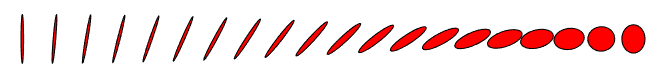
\includegraphics[width=1\linewidth]{display/1d-2x2}}\\
$X=[0,1]$, $d=2$ \\[2mm]
{
\includegraphics[width=1\linewidth]{display/1d-3x3}} \\
$X=[0,1]$, $d=3$
\end{tabular}
\end{minipage} 
\begin{minipage}[c]{.49\linewidth}
\begin{tabular}{@{}c@{}c@{}}
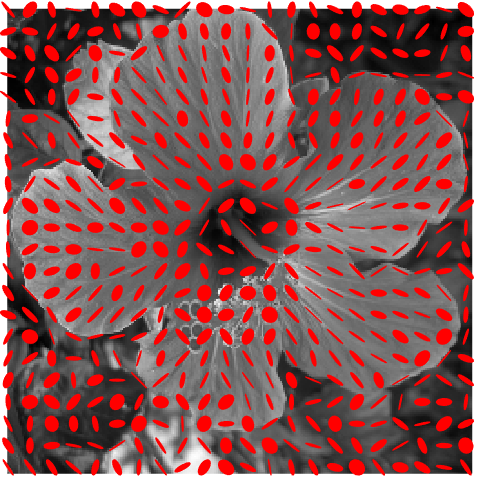
\includegraphics[width=.55\linewidth]{display/structure-tensors}&
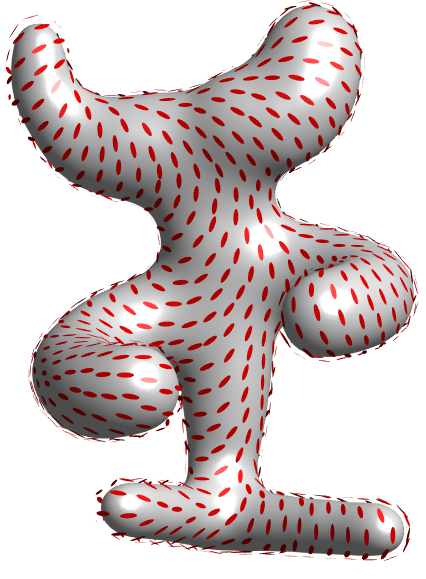
\includegraphics[width=.42\linewidth]{display/mesh}\\
 $X=[0,1]^2$ & $X=$surface \\
\end{tabular}
   \end{minipage}
\caption{Displays of various types of tensor-valued measures $\mu$. The principal directions of an ellipse at some $x_i \in X$ are the eigenvectors of $\mu_i \in \Ss_+^d$, while the principal widths are given by its eigenvalues. 
} \label{fig:display}
\end{figure}
%%%%%%%%%%%%%%%%%%%%%%%%%%%%%%%%


A tensor-valued measure $\mu$ defined on some space $X$ is a vector-valued measure, where the ``mass'' $\mu(A) \in \Ss_+^d$ associated to a measurable set $A \subset X$ is a PSD matrix. In this article, in order to derive computational schemes, we focus on discrete measures. Such a measure $\mu$ is a sum of Dirac masses
$\mu = \sum_{i \in I} \mu_i \de_{x_i}$
where $(x_i)_i \subset X$, and $(\mu_i)_i \in \Ss_+^d$ is a collection of PSD matrices. In this case, $\mu(A)=\sum_{x_i \in A} \mu_i$. 
%
Figure~\ref{fig:display} shows graphically some examples of tensor-valued measures; we use this type of visualization through the article. 
%
In the following, since the sampling points $(x_i)_i$ are assumed to be fixed and clear from the context, to ease readability, we do not make the distinction between the measure $\mu$ and the collection of matrices $(\mu_i)_i$. This is an abuse of notation, but it is always clear from context whether we are referring to a measure or a collection of matrices. 

The quantum entropy (also called von Neumann entropy) of a tensor-valued measure is 
\eql{\label{eq-h-quantum}
	H(\mu) \eqdef \sum_i H(\mu_i)
	\qwhereq 
}
\eq{
	\foralls P \in \Ss^d, \quad
	H(P) \eqdef -\tr( P \log(P)-P) - \iota_{\Ss_{+}^d}(P),
}
where $\iota_C$ is the indicator function of a closed convex set $C$, i.e. $\iota_C(P)=0$ if $P \in C$ and $\iota_C(P)=+\infty$ otherwise.
Note that $H$ is a concave function. 
%
The quantum Kullback-Leibler divergence (also called quantum relative entropy) is the Bregman divergence associated to $-H$. For a collection of PSD matrices $\mu=(\mu_i)_i, \xi=(\xi_i)_i$ in $\Ss_+^d$ corresponding to measures defined on the same grid, it is defined as %assuming $\xi_i \in \Ss_{++}^d$,
\eql{\label{eq-kl-quantum}
	\KL(\mu|\xi) \eqdef \sum_i \KL(\mu_i|\xi_i), 
}
where for all $(P,Q) \in \Ss_{+}^d \times \Ss_{+}^d$, we denote
\eq{	
	\KL(P|Q) \eqdef 
	\tr( P \log (P) - P\log (Q) - P + Q ) + \iota_{\Ss_{++}^d}(P)
}
which is convex with respect to both arguments. 
%
The inner product between collections of matrices $\mu=(\mu_i)_i, \xi=(\xi_i)_i$ is 
\eq{
	\dotp{\mu}{\xi} \eqdef \sum_{i} \dotp{\mu_i}{\xi_i} \eqdef \sum_{i} \tr( \mu_i \xi_i^\top ).
}
Given a collection of matrices $\ga=(\ga_{i,j})_{i \in I,j \in J}$ the marginalization operators read
\eq{
	\ga \ones_J \eqdef \Big(\sum_j \ga_{i,j}\Big)_i 
	\qandq
	\ga^\top \ones_I \eqdef \Big(\sum_i \ga_{i,j}\Big)_j .
}
